\documentclass{article}
\usepackage{fontspec}
\usepackage{bangla}
\setmainfont{Kalpurush}

\usepackage{amsmath}
\usepackage{amssymb}
\usepackage{tikz}
\usepackage{graphicx}
\usepackage{geometry}
\geometry{a4paper, margin=1in}

\begin{document}

% ----------------------------------------------------
% Question 48
% ----------------------------------------------------
\section*{প্রশ্ন ৪৮}

\paragraph{প্রশ্ন:} 
রাজশাহী থেকে ঢাকা এবং ঢাকা থেকে রাজশাহীর উদ্দেশ্যে নির্দিষ্ট সময় পর পর একই বেগে বাস ছেড়ে যায়। $20\text{ km/h}$ বেগে মোটরবাইক চালিয়ে এক ব্যক্তি রাজশাহী থেকে ঢাকা যাওয়ার পথে লক্ষ্য করল যে, তার অভিমুখে সামনের দিক (ঢাকা) থেকে আসা বাসগুলো প্রতি $6\text{ min}$ পর পর এবং পেছন দিক (রাজশাহী) থেকে আসা বাসগুলো প্রতি $18\text{ min}$ পর পর তাকে অতিক্রম করে। বাসগুলোর প্রকৃত বেগ এবং বাস ছাড়ার সময় ব্যবধান নির্ণয় করো। 
[Buses leave continuously at regular intervals with the same speed from Rajshahi to Dhaka and from Dhaka to Rajshahi. A person riding a motorbike at a speed of $20\text{ km/h}$ from Rajshahi to Dhaka notices that buses coming from the opposite direction (Dhaka) cross him every $6\text{ min}$, and buses coming from behind (Rajshahi) cross him every $18\text{ min}$. Find the actual speed of the buses and the time interval between consecutive bus departures.]

\begin{center}
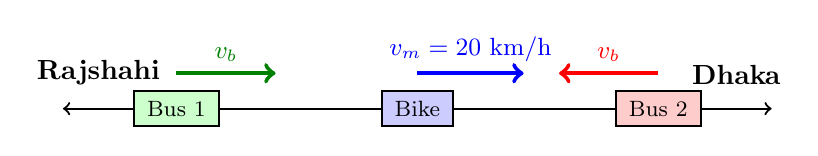
\begin{tikzpicture}[scale=0.9]
    % Road line
    \draw[thick, <->] (0,0) -- (10,0);
    \node[above, font=\bfseries] at (0.5, 0.2) {Rajshahi};
    \node[above, font=\bfseries] at (9.5, 0.2) {Dhaka};

    % Motorbike (Center)
    \draw[fill=blue!20, thick] (4.5,-0.25) rectangle (5.5,0.25);
    \node[font=\footnotesize] at (5,0) {Bike};
    \draw[->, ultra thick, blue] (5, 0.5) -- (6.5, 0.5) node[midway, above, font=\small] {$v_m = 20\text{ km/h}$};

    % Bus from Behind
    \draw[fill=green!20, thick] (1,-0.25) rectangle (2.2,0.25);
    \node[font=\footnotesize] at (1.6,0) {Bus 1};
    \draw[->, ultra thick, green!50!black] (1.6, 0.5) -- (3, 0.5) node[midway, above, font=\small] {$v_b$};

    % Bus from Front
    \draw[fill=red!20, thick] (7.8,-0.25) rectangle (9,0.25);
    \node[font=\footnotesize] at (8.4,0) {Bus 2};
    \draw[->, ultra thick, red] (8.4, 0.5) -- (7, 0.5) node[midway, above, font=\small] {$v_b$};
\end{tikzpicture}
\end{center}

\paragraph{সমাধান:}

ধরি, বাসের প্রকৃত বেগ $= v_b\text{ km/h}$ এবং বাস ছাড়ার সময় ব্যবধান $= T\text{ h}$।

দুটি বাসের মধ্যবর্তী দূরত্ব $d = v_b \times T$।

মোটরসাইকেলের বেগ $v_m = 20\text{ km/h}$।

সামনে থেকে আসা বাসের ক্ষেত্রে (বিপরীত অভিমুখে আপেক্ষিক বেগ):
$$v_{\text{rel1}} = v_b + v_m = v_b + 20$$

মিলিত হওয়ার সময় ব্যবধান $t_1 = 6\text{ min} = \frac{1}{10}\text{ h}$।
$$d = (v_b + 20) \times \frac{1}{10} \implies v_b T = \frac{v_b + 20}{10} \quad \text{--- (i)}$$

পেছন থেকে আসা বাসের ক্ষেত্রে (একই অভিমুখে আপেক্ষিক বেগ):
$$v_{\text{rel2}} = v_b - v_m = v_b - 20$$

অতিক্রম করার সময় ব্যবধান $t_2 = 18\text{ min} = \frac{18}{60}\text{ h} = \frac{3}{10}\text{ h}$।
$$d = (v_b - 20) \times \frac{3}{10} \implies v_b T = \frac{3(v_b - 20)}{10} \quad \text{--- (ii)}$$

সমীকরণ (i) এবং (ii) তুলনা করে পাই:
$$\frac{v_b + 20}{10} = \frac{3(v_b - 20)}{10}$$
$$\Rightarrow v_b + 20 = 3v_b - 60$$
$$\Rightarrow 2v_b = 80 \implies v_b = 40\text{ km/h}$$

$v_b$ এর মান সমীকরণ (i)-এ বসিয়ে পাই:
$$40 \times T = \frac{40 + 20}{10} = 6$$
$$\Rightarrow T = \frac{6}{40}\text{ h} = \frac{6}{40} \times 60\text{ min} = 9\text{ min}$$

\textbf{উত্তর:} বাসের প্রকৃত বেগ $40\text{ km/h}$ এবং বাস ছাড়ার সময় ব্যবধান $9\text{ মিনিট}$।

\vspace{1cm}
\hrule
\vspace{1cm}

% ----------------------------------------------------
% Question 49
% ----------------------------------------------------
\section*{প্রশ্ন ৪৯}

\paragraph{প্রশ্ন:} 
যদি ভেক্টর ক্ষেত্র $\vec{A} = 2x^2\hat{i} - 3yz\hat{j} + xz^2\hat{k}$ এবং স্কেলার ক্ষেত্র $\phi = 2z - x^3y$ হয়, তবে $(1, -1, 1)$ বিন্দুতে ডট গুণফল $\vec{A} \cdot \vec{\nabla}\phi$ এর মান নির্ণয় করো। 
[If vector field $\vec{A} = 2x^2\hat{i} - 3yz\hat{j} + xz^2\hat{k}$ and scalar field $\phi = 2z - x^3y$, calculate the dot product $\vec{A} \cdot \vec{\nabla}\phi$ at the point $(1, -1, 1)$.]

\begin{center}
\begin{tikzpicture}[scale=0.8]
    % 3D Coordinate Axes
    \draw[->, thick] (0,0) -- (3,0) node[anchor=west]{$y$};
    \draw[->, thick] (0,0) -- (0,3) node[anchor=south]{$z$};
    \draw[->, thick] (0,0) -- (-2.1,-1.5) node[anchor=north east]{$x$};

    % Point P(1, -1, 1)
    \coordinate (P) at (-0.7, -1, 1);
    \filldraw[black] (P) circle (2pt) node[anchor=south east] {$P(1, -1, 1)$};

    % Vectors at Point P
    \draw[->, ultra thick, red] (P) -- ++(-0.5, 2, 0.5) node[anchor=south] {$\vec{A}$};
    \draw[->, ultra thick, blue] (P) -- ++(1.2, -0.5, 0.8) node[anchor=west] {$\vec{\nabla}\phi$};
\end{tikzpicture}
\end{center}

\paragraph{সমাধান:}

প্রথমে স্কেলার ক্ষেত্র $\phi$ এর গ্রেডিয়েন্ট ($\vec{\nabla}\phi$) নির্ণয় করি:
$$\vec{\nabla}\phi = \hat{i}\frac{\partial \phi}{\partial x} + \hat{j}\frac{\partial \phi}{\partial y} + \hat{k}\frac{\partial \phi}{\partial z}$$

$$\frac{\partial \phi}{\partial x} = \frac{\partial}{\partial x}(2z - x^3y) = -3x^2y$$
$$\frac{\partial \phi}{\partial y} = \frac{\partial}{\partial y}(2z - x^3y) = -x^3$$
$$\frac{\partial \phi}{\partial z} = \frac{\partial}{\partial z}(2z - x^3y) = 2$$

$$\Rightarrow \vec{\nabla}\phi = -3x^2y\hat{i} - x^3\hat{j} + 2\hat{k}$$

$(1, -1, 1)$ বিন্দুতে $\vec{\nabla}\phi$ এর মান:
$$\vec{\nabla}\phi_{(1,-1,1)} = -3(1)^2(-1)\hat{i} - (1)^3\hat{j} + 2\hat{k} = 3\hat{i} - \hat{j} + 2\hat{k}$$

$(1, -1, 1)$ বিন্দুতে $\vec{A}$ ভেক্টরের মান:
$$\vec{A}_{(1,-1,1)} = 2(1)^2\hat{i} - 3(-1)(1)\hat{j} + (1)(1)^2\hat{k} = 2\hat{i} + 3\hat{j} + \hat{k}$$

এখন ডট গুণফল $\vec{A} \cdot \vec{\nabla}\phi$ হিসাব করি:
$$\vec{A} \cdot \vec{\nabla}\phi = (2\hat{i} + 3\hat{j} + \hat{k}) \cdot (3\hat{i} - \hat{j} + 2\hat{k})$$
$$= 2(3) + 3(-1) + 1(2) = 6 - 3 + 2 = 5$$

\textbf{উত্তর:} $5$

\vspace{1cm}
\hrule
\vspace{1cm}

% ----------------------------------------------------
% Question 50
% ----------------------------------------------------
\section*{প্রশ্ন ৫০}

\paragraph{প্রশ্ন:} 
যদি অবস্থান ভেক্টর $\vec{r} = x\hat{i} + y\hat{j} + z\hat{k}$ এবং $r = \vert{}\vec{r}\vert{}$ হয়, তবে ভেক্টর ক্যালকুলাসের আংশিক অন্তরীকরণ সূত্রাবলি ব্যবহার করে প্রমাণ করো যে, $\vec{\nabla}(\ln r) = \frac{\vec{r}}{r^2}$। 
[If position vector $\vec{r} = x\hat{i} + y\hat{j} + z\hat{k}$ and $r = |\vec{r}|$, prove using the partial differentiation rules of vector calculus that $\vec{\nabla}(\ln r) = \frac{\vec{r}}{r^2}$.]

\begin{center}
\begin{tikzpicture}[scale=0.9]
    % Axes
    \draw[->, thick] (0,0) -- (3.5,0) node[anchor=west]{$y$};
    \draw[->, thick] (0,0) -- (0,3.5) node[anchor=south]{$z$};
    \draw[->, thick] (0,0) -- (-2.1,-1.5) node[anchor=north east]{$x$};

    % Point and Position Vector
    \coordinate (P) at (1.5, 2);
    \draw[->, ultra thick, blue] (0,0) -- (P) node[midway, above left] {$\vec{r}$};
    \filldraw[blue] (P) circle (2pt) node[anchor=south west] {$P(x,y,z)$};
    
    \node[draw, dashed, inner sep=3pt] at (3.5, 1) {$r = \sqrt{x^2+y^2+z^2}$};
\end{tikzpicture}
\end{center}

\paragraph{সমাধান:}

আমরা জানি, $r = \sqrt{x^2+y^2+z^2}$।

অতএব, $\phi = \ln r = \ln(x^2+y^2+z^2)^{1/2} = \frac{1}{2}\ln(x^2+y^2+z^2)$।

এখন $\vec{\nabla}(\ln r)$ এর $x$-উপাংশটি হিসাব করি:
$$\frac{\partial \phi}{\partial x} = \frac{\partial}{\partial x}\left[\frac{1}{2}\ln(x^2+y^2+z^2)\right] = \frac{1}{2} \cdot \frac{1}{x^2+y^2+z^2} \cdot 2x = \frac{x}{x^2+y^2+z^2}$$

একইভাবে $y$ ও $z$ উপাংশদ্বয়ের জন্য আংশিক অন্তরীকরণ করে পাই:
$$\frac{\partial \phi}{\partial y} = \frac{y}{x^2+y^2+z^2}$$
$$\frac{\partial \phi}{\partial z} = \frac{z}{x^2+y^2+z^2}$$

এখন মূল গ্রেডিয়েন্ট সূত্রে মানগুলো বসিয়ে পাই:
$$\vec{\nabla}(\ln r) = \frac{\partial \phi}{\partial x}\hat{i} + \frac{\partial \phi}{\partial y}\hat{j} + \frac{\partial \phi}{\partial z}\hat{k}$$
$$\vec{\nabla}(\ln r) = \frac{x\hat{i} + y\hat{j} + z\hat{k}}{x^2+y^2+z^2}$$

যেহেতু লব $x\hat{i} + y\hat{j} + z\hat{k} = \vec{r}$ এবং হর $x^2+y^2+z^2 = r^2$, সেহেতু:
$$\vec{\nabla}(\ln r) = \frac{\vec{r}}{r^2} \quad \text{(প্রমাণিত)}$$

\end{document}